\chapter{Background}
\label{chap:background}

\textit{In this chapter, we introduce the foundation knowledge of the thesis, including the Blockchain Technology, Cryptography, and Hierarchical Deterministic Wallet (HD wallet)}

\minitoc

\section{Blockchain Technology}
\label{blockchain}
\bigskip
\subsection{What is blockchain?}

Blockchains are immutable digital ledger systems implemented in a distributed fashion (i.e., without a central repository) and usually without a central authority. The definition of blockchain was introduced to the world by a person (or a group of people) under the name Satoshi Nakamoto on October 31, 2008. It was applied to enable the emergence of a "purely peer-to-peer (no financial institution or third party) electronic cash" named Bitcoin where transactions take place in a distributed system. Satoshi did not invent the blockchain, and the Bitcoin blockchain is not the first chain that was ever created.

The word "blockchain" or "block" and "chain" wasn't used back then. Only when it was known in Satoshi Nakamoto's Bitcoin paper did the term "chain" of "blocks” become a representation for this technology. Later on, the community used that word for Nakamoto's invention. Bound to the emergence of Bitcoin and cryptocurrency, a concise description of blockchain technology is provided by NIST: Blockchains are distributed digital ledgers of cryptographically signed transactions that are grouped into blocks. Each block is cryptographically linked to the previous one (making it tamper evident) after validation and undergoing a consensus decision. As new blocks are added, older blocks become more difficult to modify (creating tamper resistance). New blocks are replicated across copies of the ledger within the network, and any conflicts are resolved automatically using established rules.

\subsection{How does it works?}


To make a blockchain work, it needs a blockchain network formed by many master nodes, a consensus protocol, and the distributed and immutable blockchain ledger. Every master node has a copy of the ledger, and most of the master nodes contribute to “validate and create” the next block to be added to the current chain to create a new ledger. By validation, that means the master node acts as a validator and confirm if a transaction is valid: is the owner of the transaction authorized, is this transaction not a double-spend one, or does this transaction follow the rules, etc. By creation, the master node each validate and put multiples valid transactions into a block, then thanks to the consensus protocols to choose whose block will be added to the chain to form a new ledger. The consensus protocol is an agreement protocol, that helps many master nodes to make a general approval on which blockchain ledger is used for the whole network and dispose of the malicious one.

Suppose that Alice wants to send 10 BTC to Bob, she uses her blockchain wallet to make a transaction, sign it, and then send the signed transaction to the blockchain network. The transaction then waits to be validated and put in a block by the master node. Now inside the blockchain network, the transaction is broadcasted to most of the master nodes to queue. Then each node can choose a number of transactions that are going to be validated and put into a block, which may contains Alice's transaction. After that, the blockchain network works on agreement which is the appropriate block to be chained with the current blockchain using consensus protocol. Bitcoin's consensus is Proof-Of-Work, in which the master node competes against each other by solving a cryptographic hash puzzle to gain the right to add their node to the chain. The puzzle must be too hard to break but fast to verify, so that the network can verify one's work and approve the new block. The first node to find out the nonce will 'mine' the block, put the validated transactions into a block with an extra transaction called coin-base transaction. The coin-base transaction is the reward for the master node, and works as incentives to encourage the node to continue to contribute to mine new blocks faithfully. That's why the term miner is born and being more common to end-users rather than master node. Once a block is mined, the node will broadcast the blockchain appended with the new block to the blockchain network. If that block contains Alice's transaction, her transaction is finished and Bob now has 10 BTC in his blockchain wallet.

\section{HD wallet}
\label{HD wallet}

\subsection{What is a blockchain wallet?}

A blockchain wallet, sometimes referred to as a cryptocurrency wallet or crypto wallet, is a program that allows you to "store", send and receive digital currencies. Since cryptocurrency doesn’t exist in any physical form, your wallet doesn't actually hold any of your coins. Instead, it tracks the transactions you made, which are stored in blockchain, and then infers your balance. Thereby, blockchain is an essential component of a blockchain wallet.

Instead of holding physical coins, a wallet has a public key and a private key. Public key is a long sequence of letters and numbers that can form the wallet address. With this, other people can send money to your wallets. It’s similar to a bank account number in which it can only be used to send money to an account. Private key is used to access the funds stored in the wallet. With this, you can control the funds tied to your wallet’s address. It works like your PIN number, you should keep it 100\% secret and secure. However, it’s worth noting that not all wallets give you sole ownership of your private key, which essentially means that you don’t have full control over your coins. As well as storing your public and private keys, crypto wallets interface with the blockchains of various currencies so that you can check your balance and send and receive funds.

\subsection{Category}

Now that you know what it is, let’s take a closer look at the five different types of wallets available, each with its own advantages and disadvantages in terms of security, ease of use, convenience and a range of other factors. The most common type of wallet out there, desktop wallets are downloaded and installed on your computer. Easy to set up and maintain, most are available for Windows, Linux and Mac, although some may be limited to a particular operating system. Many cryptocurrencies offer a desktop wallet specifically designed for their coin.

Desktop wallets provide a relatively high level of security since they’re only accessible from the machine on which they’re installed. The biggest disadvantage is that they also rely on you to keep your computer secure and free of malware, so antivirus and anti-malware software, a strong firewall and a common-sense approach to security are required to keep your coins safe. Most desktop wallets will provide you with a long string of words upon installation. These words are known as your recovery seed or sentence and map with your private key, so it’s important to store them somewhere safe in case your computer dies or you need to format the operating system and re-install your desktop wallet. Some popular desktop wallets: Electrum, Exodus, Copay.

Mobile wallets are fairly similar to desktop wallets, with the obvious difference being that they run as an app on your smartphone. Mobile wallets feature many of the same advantages and disadvantages as desktop wallets, with your private key stored on your device. Smartphone wallets are often easier to use compared to their desktop counterparts and include the ability to scan other wallet addresses for faster transactions. They also make it simpler to access your coins on the go and use cryptocurrency as part of everyday life. You will need to be extra careful about losing your smartphone, though, because there’s a risk that anyone who has access to your device might also have access to your funds. Choosing an app that allows you to back up your wallet with a 12- or 24-word passphrase is a good idea. Popular mobile wallets: Jaxx, Coinomi, Edge.

Online wallets (most often provided by exchanges but sometimes offered by third parties) are connected to the Internet and are generally the easiest to set up and use. Most only require an email address and a password to create an account, and web wallets are usually designed to provide a simple and straightforward user experience. The biggest advantages to online wallets are that they can’t be lost and that they’re accessible from any computer with an Internet connection. However, being online is unfortunately also their biggest disadvantage. Because some platforms maintain the wallets of thousands of users, they can become hot targets for hackers. It’s also important to check whether the wallet you choose lets you retain complete control of your private keys or whether they’re owned by the wallet provider. Popular web wallets: blockchain.info, MyEtherWallet, Coinbase.

Hardware wallets add another layer of security by keeping your private key on a USB stick or specially designed piece of hardware. They allow the user to plug the USB stick into any computer, log in, transact and unplug – so while transactions are carried out online, your private key is stored offline and protected against the risk of hacking. As a result, hardware wallets are widely considered to offer the most secure storage option. The biggest disadvantage of hardware wallets is that they’ll cost you. Prices vary depending on the model you choose, but they generally cost upwards of \$150. You also need to keep the device safe, but if you do lose your hardware wallet, the device itself is PIN-protected and there are usually other protective measures in place to help you recover your funds. Popular hardware wallets: Ledger Nano X, Ledger Nano S, TREZOR, KeepKey.

Paper wallets take the concept of entirely offline keys used for hardware wallets to the next logical step: simply print out your public and private keys and use that piece of paper as your wallet. As secure as they are, paper wallets are also complex and quite confusing for beginners. They’re typically only used by advanced users who want a high level of security. To transfer money to a paper wallet, you use a software wallet (any of the above mentioned) to send money to the public key printed on the sheet of paper. Most often, this is printed as a QR code for easy scanning. To transfer money from the paper wallet to someone else, you would first need to transfer money to a software wallet (by manually entering the private key into the software), and then transfer money from the software wallet to the recipient as usual. Popular paper wallets: Bitaddress.org, WalletGenerator.net.

As you’re researching and comparing a range of wallets, you’ll probably come across the terms “hot wallet” and “cold wallet”, or perhaps the concept of “cold storage”. So, what does temperature have to do with crypto storage? A wallet is hot when it's connected to the Internet. Nothing on the Internet is 100\% secure, so funds kept in a hot wallet are always at a slight risk of theft or loss from software bugs or hackers. A wallet is cold when it's safely offline and can't be deliberately or accidentally compromised over the Internet.

From an economic perspective, the wallet can be custodial (requires KYC) or non-custodial (doesn’t require KYC). Custody means that your wallet is controlled by a third party, and they need your personal information to authenticate you whenever you want to use your wallet. An example is the Binance “wallet”, or actually, the application provided by Binance. Your private keys are managed by them, which resembles a bank managing your account. Also, you have to provide your ID number, phone number, and email so that every time you want to make a transaction, the application can authenticate the right owner of the wallet. With that, you put faith in a third party to secure your funds and return them if you want to trade or send them somewhere else. While a custodial wallet lessens your responsibility, it requires you to trust in the custodian that holds your funds, which is usually a cryptocurrency exchange. On the other hand, non-custodial crypto wallets give you complete control of your keys and therefore your crypto assets. While some people store large amounts of crypto on exchange accounts, many feel more comfortable with a non-custodial wallet, which eliminates a third-party between you and your crypto. Apart from that, based on an engineering prespective, we cared about how the key is managed. We re-categorize the wallet into three main groups: hardware, software and hybrid. Hardware wallets are only connected to the internet when you need to make a transaction and you have no information about the secret keys, whereas software wallets are connected to the internet and store your secret keys. Hybrid is the combination of both hardware and software wallet, that your secret keys are stored in a secured space and are managed by the software. We will develop on a hybrid wallet as we need some information about the secret keys and need to manage the keys.

\subsection{What is a HD wallet?}

A hierarchical deterministic wallet allows you to generate and manage multiple child wallets. The HD wallet architecture consists of a pair of master private key and master public key and the management software. The software has 3 functionalities: manage the keys, check assets and transfer/deposit assets. For the keys management, the software can store and derive the child key using the CKD function to create a corresponding sub wallet for the native asset of a blockchain. By that way, we can hold multiple types of cryptocurrencies and perform cross-chain actions.

Why an HD wallet? Essentially, the HD wallet helps the user to manage multiple key pairs efficiently. As mentioned above, it is not practical for the wallet to keep track of all generated key pairs, for which each of them is used to sign a transaction. The more transactions the users make, the more key pairs they have to keep track. Instead of backing up every generated key pair, now you only need to backup the master key pair in case of HD wallet. If one of the key pairs is leaked, your wallet and crypto assets are gone. Secondly,  HD wallet offers stronger privacy than non-HD wallet because key pairs are derived automatically for every transaction. Because Bitcoin and other blockchains are public ledgers, address balances are public knowledge. However, as you have multiple addresses, others may not know which addresses are linked to you and which aren’t - provided that you haven’t shared your extended public key. Your extended public key can show all of your balances, and therefore should never be shared. Beyond privacy, HD wallet offers enhanced security because every transaction received is on a different address. Someone would need multiple private keys to access your wallet’s multiple crypto balances. So as long as you haven’t shared your extended private key, your funds should be secure. And most HD wallets make it difficult, if not impossible, to share confidential information such as your master key pair.

\section{Cryptography}
\label{cryptography}

\subsection{Elliptic curve cryptography - ECC}

Elliptic curve cryptography is a branch of public key cryptography, a.k.a asymmetric-key cryptography. An elliptic curve is defined by a curve equation built on a finite field F for coordinates. In order to understand elliptic curves, knowledge about group theory and number theory are required. In the next section, we will introduce the finite field and an interesting characteristic of the group that the elliptic curve used. Then, we explain the elliptic curve cryptography, the ECDLP and some case studies that are necessary for our thesis.

\subsubsection{Finite field \& cyclic group}

A finite field, sometimes called Galois field, is a set with a finite number of elements. Roughly speaking, a Galois field is a finite set of elements in which we can add, subtract, multiply and invert. Before we introduce the definition of a field, we first need the concept of a simpler algebraic structure, a group

\vspace{0.25cm}\textbf{Definition:} A group is a set of elements $G$ together with an operation $\circ$ which combines two elements of $G$. A group has the following properties

\begin{itemize}
  \item The group operation $\circ$ is closed. That is, for all $a,b \in G$, it holds that $a \circ b = c \in G$.
  \item The group operation is associative. That is, $a \circ (b \circ c) = (a \circ b) \circ c$ for all $a, b, c \in G$.
  \item There is an element $1 \in G$, called the neutral element (or the identity element), such that $a \circ 1 = 1 \circ a = a$ for all $a \in G$.
  \item For each $a \in G$ there exists an element $a^{-1} \in G$, called the inverse of $a$, such that $a \circ a^{-1} = a^{-1} \circ a = 1$ for all $a \in G$.
  \item A group $G$ is an Abelian group if, furthermore, $a \circ b = b \circ a$ for all $a, b \in G$.
\end{itemize}

So, a group is set with one operation and the corresponding inverse operation. If the operation is addition, the inverse operation is subtraction; and if the operation is multiplication, the inverse operation is division or multiplication with the inverse element. What we call a field is a group with all four basic arithmetic operations. A field is defined as:

\vspace{0.25cm}\textbf{Definition:} A field F is a set of elements with the following properties.
\begin{itemize}
  \item All elements of F form an additive group with the group operation “$+$” and the neutral element $0$.
  \item All elements of F except $0$ form a multiplicative group with the group operation $\times$ and the neutral element $1$.
  \item When the two group operations are mixed, the distributivity law holds, i.e., for all $a, b, c \in F: a \times (b+c) = (a \times b) + (a \times c)$.
\end{itemize}

In the elliptic curve, we are interested in fields with a finite number of elements, the finite field. The number of elements in the field $F_p$ is called the order (cardinality) of the field, denoted by $|F_p|$. A field with order $m$ only exists if $m$ is a prime power, i.e., $m = p^n$, for some positive integer $n$ and a prime integer $p$. $p$ is called the characteristic of the finite field, denoted as $char(p)$. A finite field is denoted as $GF(p^n)$ or $F_{p^n}$. The most intuitive examples of finite fields are fields of prime order with $n = 1$. Elements of the prime field $F_p$ can be represented by integers $0, 1, …, p-1$. The two operations of the field are modular integer addition and integer multiplication modulo $p$. With $n > 1$, the field is called extension field, the elements are polynomials $a_{n-1}X^{n-1} + a_{n-2}X^{n-2} + … + a_1X + a_0$, where the coefficient $a$ is in $F_p$. The arithmetic operations in an extension field are polynomial addition modulo $p$ with the coefficients and polynomial multiplication modulo $P(x)$. $P(x)$ is called the irreducible polynomials, which acts like ‘a prime’ of the polynomials.

Elliptic curve usually works in the prime field, to gain a finite number of curve points. The points on an elliptic curve over $F_p$ also belong to a group, called cyclic group. A cyclic group is a multiplicative group $F_p^* = {gcd(x,p) = 1 | x \in {1, 2, ..., p-1}}$, where $p$ is a prime and contains at least one special element $\alpha$. The element $\alpha$ is called primitive element or generator, such that $ord(\alpha) = |(F_p)^*|$, where the order of $\alpha$ ($ord(\alpha)$) is the smallest positive integer $k$ satisfies $a^k = a \circ a \circ … \circ a$ (k times) $= 1$. The multiplies of $\alpha$ generates all the elements in the $F_p^*$ , and they repeat cyclically similar to a modulo congruence. E.g.: For a $F_{11}^*$ with order of 10, the generator $\alpha$ can be 2 since.

\setlength{\columnsep}{4cm}
\begin{multicols}{2}
  $\alpha^1 \mod 11 = 2$
  $\alpha^2 \mod 11 = 4$
  $\alpha^3 \mod 11 = 8$
  $\alpha^4 \mod 11 = 5$
  $\alpha^5 \mod 11 = 10$
  $\alpha^6 \mod 11 = 9$
  $\alpha^7 \mod 11 = 7$
  $\alpha^8 \mod 11 = 3$
  $\alpha^9 \mod 11 = 6$
  $\alpha^{10} \mod 11 = 1$
  $\alpha^{11} \mod 11 = 2$
  $\alpha^{12} \mod 11 = 4$
  $\alpha^{13} \mod 11 = 8$
  And so on...
\end{multicols}


Note that there can be more than one generator for a cyclic group, but a group only needs one element $\alpha$ to be cyclic. It is similar to a finite field, with an additional condition, that is the element $\alpha$. This behavior will also work for an elliptic curve introduced in the next section, where the scalar multiples of a point on an elliptic curve are repeating cyclically.

\subsubsection{Weierstrass curve - the general form of an elliptic curve}
About elliptic curves, there are curve types and equation types. An elliptic curve $E$ defined over a field $F_p$ is given by the equation

\hspace{0.25cm}
\begin{center}
  $y^2 + a_1xy + a_2y \equiv x^3 + a_3x^2 + a_3x^2 + a_4x + a_5 \quad (mod \quad p)$\\
\end{center}
\hspace{0.25cm}

where the coefficients $a_i$ are elements in the field $F_p$. The set of points in $E(F_p)$ satisfied the equation and the point of infinity $\Theta$. The elliptic curves that satisfy the equation above are called Weierstrass curves, i.e., a curve type. Consider polynomials over $F_p$, where a characteristic $char(p) \neq 2,3$, the equation above can be reduced into a short Weierstrass form

\hspace{0.25cm}
\begin{center}
  $y^2 \equiv x^3 + a_1x + a_2 \quad (mod \quad p)$, where $4a_1^3 + 27a_2^2 \not\equiv 0 \mod p$
\end{center}
\hspace{0.25cm}

The set of all pairs $(x,y) \in F_p$ together with an imaginary point at infinity $\Theta$ satisfying the equation is the set of points on the elliptic curve, with the condition to exclude singular curve. The scalar multiplication, addition and doubling laws allow arithmetic operations in the elliptic curve group laws. The group laws for an elliptic curve

\begin{itemize}
  \item The elements of the group are the points of an elliptic curve.
  \item The neutral element is the point at infinity $\infty$, denoted $\Theta$.
  \item The inverse of a point $P$ is the one symmetric about the x-axis.
  \item Addition is given by the rule: given three aligned, non-zero points $P$, $Q$, and $R$, their sum is $P + Q + R = \Theta$.
  \item The inverse or negative point of a point $P(x,y)$ is defined as $-P(x,y) = P(x,-y)$ such that $P + (-P) = \Theta$.
\end{itemize}

The set of points on the elliptic curve with the point $\Theta$ has cyclic subgroups. Under certain conditions all points on an elliptic curve form a cyclic group. Each point on an elliptic curve is a generator for its cyclic subgroup of point on $E$. As mentioned above, an element $\alpha$ now is a point on the curve, it may not generate all point on a curve but its generated group is a cyclic subgroup, i.e., part of all points on the curve. The ECC works around this special case in ECDLP.

The point arithmetic operations defined in the group law are in geometric representation. To work with $F_p$, point addition laws need to be calculated in an algebraic way. The addition laws for a general curve, given $P(x_1, y_1), Q(x_2, y_2), R(x_3, y_3)$, are

\begin{itemize}
  \item $P + \Theta = \Theta + P = P$
  \item $\Theta + \Theta = \Theta$
  \item $P + Q = \Theta$ if $Q = -P$ or $P = -Q$
  \item If $P \neq Q$, $P + Q = R$, the coordinates of $R$ can be computed as

        \begin{itemize}
          \item[$\bullet$] Compute $s = (y_2 - y_1) (x_2 - x_1)^{-1} \mod p$
          \item[$\bullet$] Compute $x_3 = s^2 - x_1 - x_2 \mod p$, and $y_3 = s(x_1 - x_3) - y_1 \mod p$
        \end{itemize}

  \item If $P = Q$, $P + Q = P + P = 2P = R$, the coordinates of $R$ can be computed as

        \begin{itemize}
          \item[$\bullet$] Compute $s = (3x_1^2 + a_1 (2y_1)^{-1} \mod p$
          \item[$\bullet$] Compute $x_3 = s^2 - 2x_1 \mod p$, and $y_3 = s(x_1 - x_3) - y_1 \mod p$
        \end{itemize}

\end{itemize}

Here, the addition law is incomplete, since we can’t add the same point twice, we have to use the point doubling formula. The Weierstrass form is the general form of an elliptic curve, any curve can be expressed in a Weierstrass form. There are also other types of curves such as the Koblitz curve, Montgomery curve and (twisted) Edwards curve, which will be presented in the following sections. Before that, most of the elliptic curves need a domain parameter as follow.\\

\begin{itemize}
  \item$p$: The prime that specifies the size of the finite field
  \item$a, b$: The coefficients of the elliptic curve equation in (short) Weierstrass form
  \item$N$: the order of the elliptic curves ($\#E$)
  \item $P$: a point on the elliptic curve
        \item$G$: The base point that generates our subgroup
        \item$n$: The order of the subgroup (which is the order of the basepoint $G$). $n$ must be prime
        \item$h$: The cofactor of the subgroup such that with $n(hP)=0$, $G = hP$. In other words, $h=N/n$
\end{itemize}

Also, in practice, a point $P(x,y)$ can be compressed to an integer ($y$’s LSB in the first byte $\|$  $x$). The first byte of $y$ can be $0x02$ for even $y$, or $0x03$ for odd $y$(negative $y$) with the given $x$. For instance, a point $P(6, 8)$ can be compressed to the integer $0x026$ in hexadecimal format. The actual number is almost 256-bit long, this is just a simple example.

\subsubsection{Elliptic curve discrete logarithm problem - ECDLP}

Given an elliptic curve $E$, we consider a primitive element $P$ and other element $T$, the discrete log problem is finding an integer $d$, where
\begin{center}

$d \in [1, \#E]$ such that $P + P + … + P$ ("+" $d$ times) $= dP = T$.
\end{center}

The ECDLP is considered to be infeasible if the elliptic curve parameters are carefully chosen \cite{DBLP:journals/iacr/BosCLN14}. In ECC, we interpret the integer $d$ as the private key, $T$ as the public key, and the exact number of point points $E$ of a curve. The number of points on the curve can be counted by trying all the possible values for $x$ in $F_p$, but this is not efficient if the $p$ is a large prime. Haskel’s theorem only gives an upper and lower bound for number of point on an elliptic curve parameters are carefully chosen \cite{DBLP:journals/iacr/BosCLN14}. 

\hspace{0.25cm}
\begin{center}
  $p+1-2\sqrt{p} \leq \#E \leq p+1+2\sqrt{p}$\\
\end{center}
\hspace{0.25cm}

In order word, find the exact numbers of points on a curve is computationally difficult. Luckily, there's a faster algorithm for computing the order: Schoof's algorithm. We won't enter the details of the algorithm - what matters is that it runs in polynomial time, and this is what we need.

\subsubsection{Koblitz curve, case study: Secp256k1}
The elliptic curve Secp256k1 is a Koblitz curve, which has the equation

\hspace{0.25cm}
\begin{center}
  $y^2 \equiv x^3 + 7 \quad (mod \quad p)$
\end{center}
\hspace{0.25cm}

with the param standards \href{https://en.bitcoin.it/wiki/Secp256k1}{Secp256k1}, where $p = 2^{256 - 232 - 29 - 28 - 27 - 26 - 24 - 1}, h = 1$. Its finite field is defined over the finite field $F_2$, with the neutral element as the point at infinity $\Theta$. The addition law for Secp256k1 are \href{https://www.researchgate.net/publication/332783847_Arithmetic_of_Koblitz_Curve_Secp256k1_Used_in_Bitcoin_Cryptocurrency_Based_on_One_Variable_Polynomial_Division}{Secp256k1 documentaton} and improved in \href{https://www.researchgate.net/publication/223346975_Koblitz_curve_cryptosystems}{Koblitz curve cryptosystem} .The addition law for the Koblitz curve is “incomplete”.

\subsubsection{Montgomery curve, case study: Curve25519}
Daniel J. Bernstein originally discovered the Curve25519, in the form of the Montgomery curve, has the equation

\hspace{0.25cm}
\begin{center}
  $By^2 \equiv x^3 + A^2 + x \quad (mod \quad p)$, where $B(A^2-4) \neq 0, B \neq 0, A \neq \pm 2$
\end{center}
\hspace{0.25cm}

with $A = 486662x, B = 1$, over the prime field defined by the prime number $p=2^{255}-19$, the base point has $x$-coordinate $= 9$,  the cofactor $h = 8$ and the subgroup order is $n = 2^{252} + 27742317777372353535851937790883648493$. The neutral element is the point at infinity $\Theta$, and the negation is $-P(x, y) = P(x, -y)$. The Montgomery curve has a special algorithm to compute scalar multiples of points in constant-time, called Montgomery ladder. Let the scalar integer is $a$ in binary form and the point is $P$, the algorithm works as follow

\begin{figure}[ht!]
  \centering
  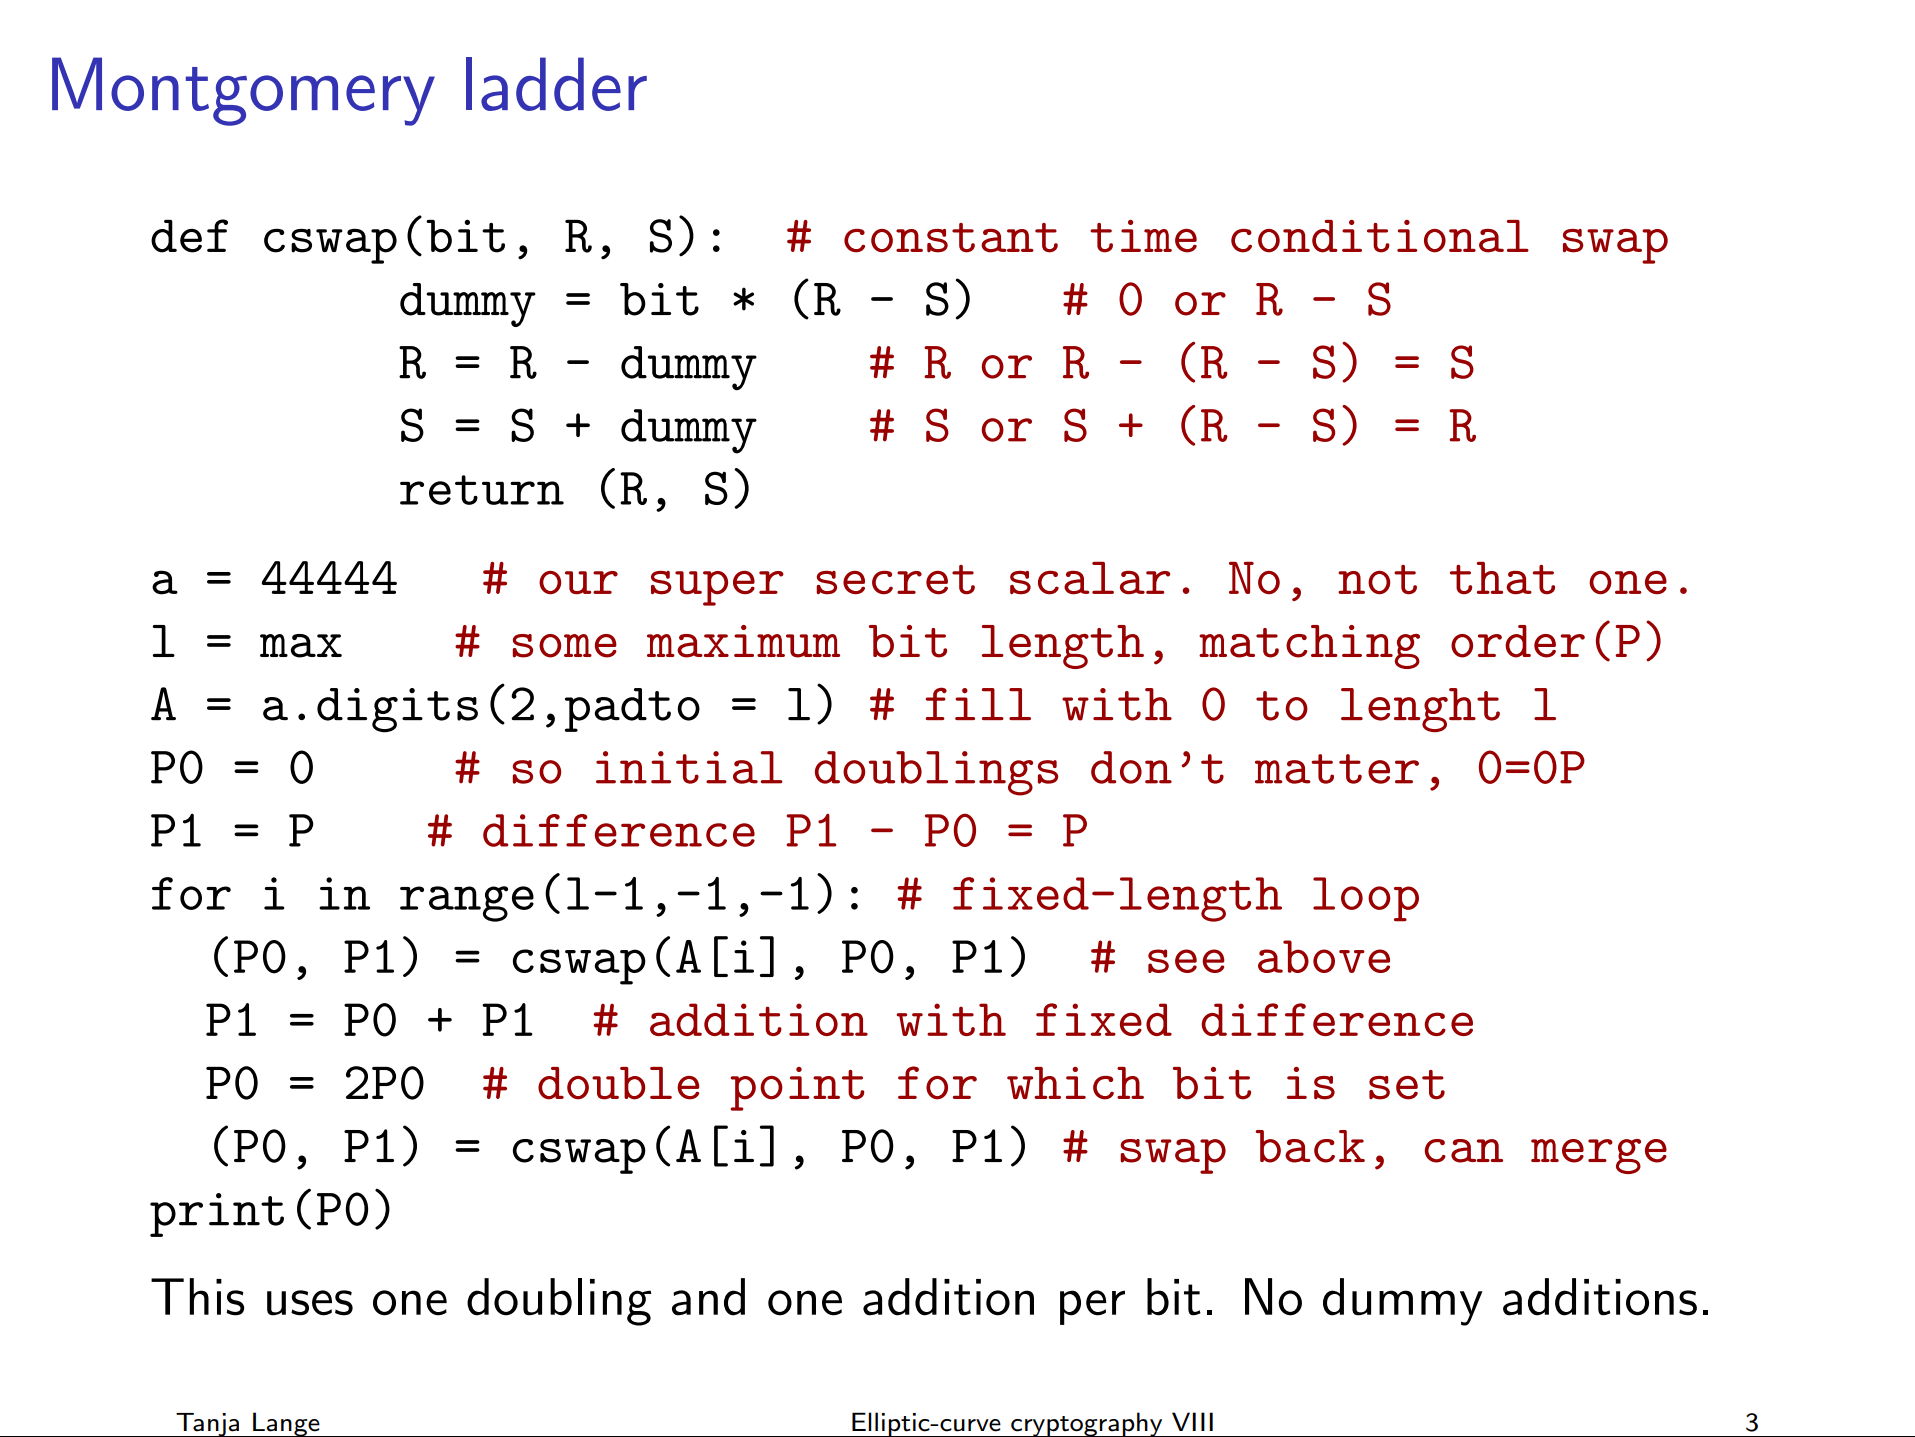
\includegraphics[width=0.6\textwidth]{images/montgomery_ladder.png}
  \caption[Montgomery ladder]{Montgomery ladder}
  \label{fig:montgomery_ladder}
\end{figure}

\begin{itemize}
  \item Assign initial value for $P_0 = 0$ and $P_1 = P$ so initial doublings don’t matter $(P_0 =0P$, $2*0P = 0P)$ and $P_1$ is the difference $P_1 - P_0 = P$
  \item Assign initial value for $P_0 = 0$ and $P_1 = P$ so initial doublings don’t matter $(P_0 =0P, 2*0P = 0P)$ and $P_1$ is the difference $P_1 - P_0 = P$

        \begin{itemize}
          \item[$\bullet$] If the bit is 0 compute $P_1 = P_0 +  P1$ and $P_0 = 2P_0$
          \item[$\bullet$] Else the bit is 1 $P_0 = P_0 +  P_1$ and $P_1 = 2P_1$
        \end{itemize}

  \item The final result of $[a]P$ is $P_0$
\end{itemize}

Montgomery ladder always performs doubling and adding in the algorithm, allowing the time cost to be constant. It works since the Montgomery curve always has the point (0, 0) of order 2 (assignable to $P_0$). Also, the addition laws for Montgomery, given $P(x_1, y_1), Q(x_2, y_2), R(x_3, y_3)$, are

\begin{itemize}
  \item $P + \Theta = \Theta + P = P$
  \item $\Theta + \Theta = \Theta$
  \item $P + Q = \Theta$ if $Q = -P$ or $P = -Q$
  \item If $P = Q$ and $x_1 = x_2 \neq 0$, the coordinates of $R$ can be computed as

        \begin{itemize}
          \item[$\bullet$] Compute $s = (3x_1^2 + 2Ax_1 + 1) (2By_1)^{-1} \mod p$
          \item[$\bullet$] Compute $x_3 = Bs^2 - A - 2x_1 \mod p$, and $y_3 = s(x_1 - x_3) - y_1 \mod p$
        \end{itemize}

  \item If $P = Q$, $P + Q = P + P = 2P = R$, the coordinates of $R$ can be computed as

        \begin{itemize}
          \item[$\bullet$] Compute $s = (y_1 - y_2) (x_1 - x_2)^{-1} \mod p$
          \item[$\bullet$] Compute $x_3 = Bs^2 - A - x_1 - x_2 \mod p$, and $y_3 = s(x_1 - x_3) - y_1 \mod p$
        \end{itemize}
\end{itemize}

\subsubsection{Edwards curve and the twisted Edwards curve, case study: Edwards25519}

The Curve25519 can be transformed to twisted Edwards form (from here, we refer to Curve25519 in twisted Edwards form as Edwards25519). The curve Edwards25519 has the equation

\hspace{0.25cm}
\begin{center}
  $ax^2 + y^2 \equiv 1 + dx^2 y^2 \quad (mod \quad p)$
\end{center}
\hspace{0.25cm}

with the same prime field $p$ and the cofactor $h$. Edwards25519 has some additional parameters:

\begin{itemize}
  \item $b = 256$, the bit length of the coordinate satisfies $2^{b-1} > p$
  \item A non-square $d: -121665/121666$
  \item A non-zero $a$: if $a = 1$, it's a normal Edwards curve, else it's a twisted Edward curve ($a = -1$ for Edwards25519)
  \item An odd prime $L$ (same as n in a general elliptic curve), where $h \times L = \#E: 2^{252}+27742317777372353535851937790883648493$ (\~253 bits)
  \item The basepoint $B$: $B(x, 4/5) \neq (0, 1)$ with positive $x$
\end{itemize}


The neutral element is $\Theta = (0,1)$, and the negation is $-P(x, y) = P(-x, y)$. Note that Curve25519 and Edwards25519 are birational equivalence (proved in \cite{Bernstein2011}). Therefore; Edwards25519 also supports Montgomery ladders. The Edwards25519 uses a point encoding scheme rather than a standard point compression. A point $P(x, y)$ is presented as a 32-octet string, interpreted as a little-endian integer. To encode a point $P(x, y)$\\

\begin{itemize}
  \item Encode the y-coordinate as a little-endian string of 32 octets. The MSB of the last octet is always zero.
  \item Copy the LSB of the x-coordinate to the MSB of the last octet string.
        Resulting in an encoded point with 256 bits length, with the 256-bit to be the LSB of $x$, called $x_0$. To decode a point, it takes more works than encoding
  \item Clearing the $x_0$ - the MSB of the octet string to obtain $y$. If $y \geq p$, decoding fails
  \item $x$ can be retrieved by computing $x^2 = (y^2 - 1)/(dy^2 + 1) \mod p$
  \item Denote $u = (y^2-1), v = (dy^2 + 1)$, $w$ is the candidate root. Calculate $w = uv^3(uv^7)^{(p-5)/8} \mod p$
  \item There are three cases

        \begin{itemize}
          \item[$\bullet$] If $vw^2 = u \mod p, x = w$
          \item[$\bullet$] If $vw^2 = -u \mod p, x = w \times 2^{(p-1)/4}$
          \item[$\bullet$] Otherwise, no square root exists. Decoding fails
        \end{itemize}

  \item If $x = 0,x_0 = 1$, decoding fails. Else, if $x_0 = x \mod 2$ then $x = x$, if not then $x = p - x$
\end{itemize}

The main reason for point encoding is for security (same as point compression) performance (will be explained in Ed25519). The addition laws for twisted Edwards curve are always, given $P(x_1, y_1), Q(x_2, y_2)$:

\hspace{0.25cm}
\begin{center}
  $(x_1, y_1) + (x_2, y_2) \equiv \left(\cfrac{x_1y_2 + x_2y_1}{1 + dx_1x_2y_1y_2}, \cfrac{y_1y_2 - ax_1x_2}{1 - dx_1x_2y_1y_2}\right) \quad (mod \quad p) $
\end{center}
\hspace{0.25cm}

which means that the addition laws for twisted Edwards are complete (no exception cases, as long as the parameters $a$ and $d$ follow their condition above).

\subsection{Digital signature with ECC}

\subsubsection{The standard ECDSA}
ECDSA is a standard Digital Signature Algorithm for elliptic curve cryptography. The necessary parameters are defined above, with a hash function $H$ and the message $M$ needs to be signed. Denote that $k$ is the randomly generated private key in the range  $[1, n - 1]$, and $K$ is the public key by a scalar multiplication $K =[k]G$. To sign a message, do the following steps:

\begin{itemize}
  \item Choose a random integer $a$ from $[1, n - 1]$ (called nonce)
  \item Calculate $P = [a]G = (x, y)$, then $r = x \mod n$. If $r = 0$, goes back to step 1
  \item If not, calculate $s=(m+rk) a^{-1} \mod n$,with $m = H(M)$ as the hash value of the message. If $s = 0$, goes back to step 1
  \item If not, the pair $(r, s)$ is the signature.
\end{itemize}

The process requires choosing an appropriate random integer $a$ to mask the private key through the modular multiplicative inverse of $a$ and the sum of $m$ with $r$ times $k$. To verify the signature, we re-calculate point $P’$ and compare the x-coordinate:

\begin{itemize}
  \item Calculate $u = s^{-1}m \mod n, v = s^{-1}r \mod n$
  \item Calculate $P' = [u]G + [v]K = (x', y')$
  \item Compare $r$ and $(x' \mod n)$; if they are congruent, the signature is valid
\end{itemize}

The algorithm’s proof of correctness

\begin{itemize}
  \item $P’ = [u]G + [v]K = [u]G + [vk]G = [u +vk]G = [s^{-1}m \mod n + s^{-1}rk \mod n]G = [s^{-1}(m + rk) \mod n]G$ (1)
  \item Since $s = a^{-1}(m+rk) \mod n \Rightarrow a = s^{-1}(m+rk) \mod n$ (2)
  \item Substitute (2) into (1), $P’ = [s^{-1}(m + rk) \mod n]G = [a]G = P$
\end{itemize}

The verification is simple to understand, but note that we have to calculate modular multiplicative inverse in both processes, signing and verifying. The modular inverse is an expensive ECC computation. In modular arithmetic, to find a multiplicative inverse of an integer $a$ with a prime $p$, we first compute if $gcd(a, p) = 1$ to know If $a$ has a modular inverse. ECC requires one more condition compared to modular arithmetic: the point needs to be on the curve, which means the coordinates have to satisfy the curve equation and follow the curve’s addition law. That’s why signing a message takes a lot of trial and error to find a suitable nonce. Moreover, to ensure the private key won’t be leaked, the nonce has to be randomly generated for every signature. Or else, the private key can be retrieved as follow

\begin{itemize}
  \item Assume that the signature $s_1$ and $s_2$ use the same nonce, which means $r_1 = r_2 = r$. The hash values of the two messages are $H(M_1) = m_1 and H(M_2) = m_2$.
  \item $s_1 - s_2 = a^{-1} (m_1 + rk) - a^{-1} (m2+rk) \mod n$
  \item $s_1 - s_2 = a^{-1}(m_1 + rk - m_2 - rk) \mod n$
  \item $s_1 - s_2 = a^{-1}(m_1 - m_2) \mod n$
  \item $a = (m_1 - m_2)(s_1 - s_2)^{-1} \mod n$, the attacker now retrieves the nonce
  \item Since $s = a^{-1}(m + rk) \mod n \Rightarrow k = (sa-m) r^{-1} \mod n$, simply substitute nonce $a$ into the equation, the attacker can access your private key.
\end{itemize}

This error has been exploited in the real-world, et al \href{https://events.ccc.de/congress/2010/Fahrplan/attachments/1780_27c3_console_hacking_2010.pdf}{Console Hacking 2010 - PS3 Epic Fail Archived} December 15, 2014, at the \href{https://en.wikipedia.org/wiki/Wayback_Machine}{Wayback Machine}, page 123-128. Because Sony uses a static nonce for every signature, the private key was extracted, thereby gaining the public key required to run any software on the machine.


\subsubsection{Schnorr’s signature scheme and EdDSA}

EdDSA is a digital signature scheme using a variant of Schnorr’s signature based on twisted Edwards curves. Originally, the standard Schnorr’s signature algorithm for an elliptic curve includes these steps

\begin{itemize}
  \item Choose a private key $k$ in range $[1, n -1]$ and calculate $P = [k]G$
  \item Hash the message $M$ to obtain $m = H(M)$
  \item Generate a random number $z$ in range $[1, n -1]$, then calculate $R = [z]G$
  \item Calculate $s = z + H(r \| P \| m) \times k$, where $r$ is the x-coordinate of the point $R$, $\|$ denote string concatenation
  \item The signature is the pair $(r, s)$
\end{itemize}

Once you obtain the signature $(r, s)$ and the public key (the point $P$), you can verify it by

\begin{itemize}
  \item Calculate $R(r, y)$ with $r$
  \item Verify if $[s]G = R + [H(r \| P \| m)]P$. If true, the signature is valid
\end{itemize}

Proof of correctness

\begin{itemize}
  \item LHS: $[s]G = [z + H(r \| P \| m) \times k]G$
  \item RHS: $R + [H(r \| P \| m)] P = [z]G + [H(r \| P \| m)] \times [k]G = [z]G + [H(r \| P \| m) \times k]G = [z + H(r \| P \| m) \times k]G = LHS$
\end{itemize}

Schnorr’s signature algorithm, therefore, guarantees that if either $r$, the original message $m$, or the public key $P$ is invalid, the signature is also invalid. Note that a point is compressed when hashing, with a corresponding compression scheme for the curve. Then, in 2012, Daniel J. Bernstein, Niels Duif, Tanja Lange, Peter Schwabe, and Bo-Yin Yang adjusted Schnorr’s signature for twisted Edwards curve and developed an EdDSA scheme, called Ed25519. Since Ed25519 use a point little-endian encoding scheme, the key generation is a bit different

\begin{itemize}
  \item Private key: a $b$-bit randomly generated integer $k$
  \item Public key: also a $b$-bit integer. To generate a public key from the private key

        \begin{itemize}
          \item[$\bullet$] Hash the private key: $H(k) = (h_0, h_1,…, h_{2b-1})$
          \item[$\bullet$] Use the lower 32 bytes $(h_0, h_1,..., h_{b-1})$ for buffer. Pruning the buffer by setting $h_0 = h_1 = h_2= h_{b-1} = 0$, and $h_{b-2} = 1$
          \item[$\bullet$] Interpret the buffer as a little-endian integer, denoted $s$
          \item[$\bullet$] Computer the point $A’ = [s]B$
          \item[$\bullet$] Encode $A’$ to obtain $A$. $A$ is the public key
        \end{itemize}

\end{itemize}

To sign a message $M$, you need the private key $k$ and the public key $A$. The steps are

\begin{itemize}
  \item Hash the private key:  $H(k) = (h_0, h_1 ,…, h_{2b-1})$
  \item Use the higher 32 bytes $(h_b, h_{b+1},..., h_{2b-1})$ for buffer
  \item Compute $r = H($ buffer $\| M) \mod L$
  \item Compute $R’ = [r]B$ and encode $R’$ to gain $R$
  \item Compute $s$ (the same as public key generation). Then compute and encode to obtain the public key $A$
  \item Compute $e = H(R\|A\|M) \mod L$
  \item Compute $S’ = (r+e \times s) \mod L$, encode $S’$ to obtain $S$
  \item The signatures is $(R \| S)$
\end{itemize}

Note that $S$ is the little-endian encoding of $S’$, which has the three MSB of the final octets are always zero. This causes the last 3 bits of the signature $(R \| S)$ are also zeros. For verification, any decoding failure means that the signatures are invalid. To verify the signature $(R \| S)$\\

\begin{itemize}
  \item Decode the first half (the first 256 bits) of the signature for $R’$ and the other half for $S’$
  \item Decode $A$ to obtain $A’$
  \item Compute $e’ = H(R\|A\|M)$ as a 64-byte little-endian integer
  \item If $[S’]B = R’ + [e’]A’$, then the signature is valid
\end{itemize}

Take a note that $e’$ (512-bit) is congruent to $e$(253-bit) mod $L$, which means the scalar multiplication will result in the same point. Proof-of-correctness

\begin{itemize}
  \item LHS = $[S]B = [(r + e \times s) \mod L]B = [r \mod L]B + [e \times s \mod L]B = [r]B + [e \times s]B = R’ + [e]A’$
  \item As noted, $[e’]P = [e]P \Rightarrow [e’]A’ = [e]A’$ (1)
  \item Substitute (1) into LHS = $R’ + [e]A’ = R’ + [e’]A’$ = RHS
\end{itemize}

In EdDSA, we can see that there is no random nonce used. Instead, EdDSA uses a deterministic nonce from the message digest and a part of the private key. Through all the process, the private key is not used directly to sign, ensure that there are no information about the private key can be leaked.

\subsection{Comparison between ECDSA with Secp256k1 and Ed25519}

\subsubsection{Secp256k1 vs. Ed25519}

For ECC, we consider a curve is secure based on these criteria (according to \href{http://safecurves.cr.yp.to/index.html}{SafeCurve}): the curve’s resistance to the attacks on the elliptic curve discrete logarithm (ECDLP security) and its resistance to attack in the real world (ECC security). SafeCurve did list some of the criteria for ECDLP, but M. C. Semmouni, A. Nitaj and M. Belkasmi in \href{https://sci-hub.se/10.1080/09720529.2019.1681673}{Bitcoin security with a twisted Edwards curve} had conducted more thorough research on the cryptanalytical study and the efficiency analysis to point out that Edwards25519 is more secure than the curve Secp256k1. First of all, they reviewed the ECDLP for each curve in terms of complex-multiplication field discriminants, Pohlig - Hellman attack, Pollard’s rho attack (with j-invariant for speedup), anomalous attack, Frey-Ruck attack, and MOV supersingular attack. Their work proved that Edwards25519 is more resistant than the curve Secp256k1 to two attacks, which are complex-multiplication field discriminants and Pollard’s rho. Secondly, to analyze the efficiency of Edwards25519 and the curve secp256k1, they compared the curves’ arithmetical operations over projective coordinates. To evaluate the computational cost, let denote multiplication as M, squaring as S, addition as Add, and doubling as D. All the operations are performed in modular arithmetic, assuming that 1S = 1M (multiply by itself), 1D = 2Add. They pointed out that the computational cost on the curve secp256k1 takes 12M + 4S + 1D + 6Add (= 16M + 8Add) for point addition and 3M + 6S + 8D + 5Add (= 9M + 21Add) for point doubling. Whereas, the computational cost on Edwards25519 takes up to 7M + 2D + 7Add (= 7M + 11Add) for point addition and up to 3M + 4S + 1D + 6Add (= 7M + 8Add) for point doubling. It’s clear that the operations on Edwards25519 are faster than those on the curve Secp256k1. They concluded that “it is more convenient to use the curve Edwards25519 for industrial applications such as in a Bitcoin system”.

On the other hand, the requirements for ECC security are ladders \href{http://safecurves.cr.yp.to/ladder.html}, completeness \href{http://safecurves.cr.yp.to/complete.html}, and indistinguishability \href{http://safecurves.cr.yp.to/ind.html}. Ladders require a curve’s single-scalar multiplication to be time-constant. Single-scalar multiplication is the most necessary computation in ECC (computing the curve point $[n]P$ given an integer $n$ and a curve point $P$, which is the bottleneck in key generation, signing, and key exchanges. If the multiplication doesn’t take constant time, the attackers can perform a timing attack to find out the secret keys. In 2014, Naomi Benger and Joop van de Pol and Nigel P. Smart and Yuval Yarom published a paper explaining how to recover secret keys from OpenSSL's implementation of ECDSA-secp256k1 using timing information from "as little as 200 signatures". They were able to make use of the side-channel information from almost all of the observed executions and succeeded in recovering the private key. To avoid the leakage of side-channel timing information, a safe curve has to support ladders.  As mentioned above, any curve that is birationally equivalent to Montgomery form is ladder supported. The Koblitz curve Secp256k1 uses a different finite field, which lacks the point (0, 0) and its order is not divisible by 4, causing it can be isomorphic to neither the standard Weierstrass form nor Montgomery form. On the contrary, Edwards25519 is birationally equivalent to the Montgomery form of Curve25519, which allows it to have the ladder by default. Secondly, completeness means that a curve’s addition law must have no exceptions, which means that for every rational point $P$ on $E$ and every rational point $Q$ on $E$, the addition law for inputs $P$ and $Q$ produces exactly outputs $P + Q$. Secp256k1 has a special case for adding the same point, adding with negation and adding with the infinity point  (i.e., they have cases for adding the point at infinity, adding the point twice,...), while Edwards25519’s addition law is proven to be complete. Finally, indistinguishability is short for “indistinguishability from uniform random strings”. Standard representations of elliptic-curve points are easily distinguishable from uniform random strings. This poses a problem for many cryptographic protocols using elliptic curves: censorship-circumvention protocols, for example, and password-authenticated key-exchange protocols. 2013 Bernstein–Hamburg–Krasnova–Lange introduced the following solution to the underlying problem. Construct an efficient constant-time bijective map between a large set of $b$-bit strings (large enough to be indistinguishable from all $b$-bit strings; i.e., very close to $2^b$ possibilities) and a large set of rational points on an elliptic curve (e.g., about half of all points). Use uniform random points in this set, and represent them by the corresponding strings under this bijective map. These strings are indistinguishable from uniform random $b$-bit strings. There are various requirements for a curve to be able to construct a map, such as a subgroup order has to be congruent to $3 \mod 4$ or multiple of $4$, but Secp256k1 fails these requirements. Overall, Edwards25519 does pass the core requirements of a curve to be “safe” enough to be applied in the real-world ECC in comparison to Secp256k1.


\subsubsection{ECDSA vs. Ed25519}

To evaluate these two digital signature schemes, we will analyze their algorithm and benchmark the time required for key generation, signing, and verifying. ECDSA is the standard DSA for elliptic curve cryptography based on the ElGamal. The signature digital scheme Ed25519 is a variant of Schnorr’s signature algorithm based on twisted Edwards curves. The hash functions used in each signature scheme are different: SHA-256 for ECDSA and SHA-512 for Ed25519. They differ only in the input bit lengths and produce outputs of lengths of 256 bits and 512 bits respectively. Nevertheless, SHA-256 and SHA-512 don’t have the same security level. SHA-512 is more secure than SHA-256 and is recommended by various cryptographic standards such as \href{https://csrc.nist.gov/projects/hash-functions/nist-policy-on-hash-functions}{Policy on Hash Functions}, \href{https://www.enisa.europa.eu/publications}{ENISA: Algorithms, key size and parameters report (2014)} and \href{https://www.keylength.com/en/}{BlueKrypt, cryptographic key length recommendation} for use for more sensitive data and for longest terms. This is an advantage for the digital signature Ed25519 over the digital signature ECDSA for long terms. Also, in the case of Ed25519, it chooses the nonce deterministically as the hash of a part of the private key and the message rather than a randomly generated nonce for each signature. Therefore; as long as the generated private key is secure, Ed25519 has no further need for a random number generator in order to make signatures, and there is no danger that a broken random number generator used to make a signature will reveal the private key.

For benchmarks, we found some awesome repo on github: \href{https://github.com/justmoon/curvebench}{justmoon}, the Rust implementation of Ed25519 \href{https://github.com/dalek-cryptography/ed25519-dalek}{dalek}, and the Rust implementation of Secp256k1 (tarcieri). In justmoon repo, he ran the original implementation of both algorithms, which produced a \href{http://justmoon.github.io/curvebench/benchmark.html}{result} of Ed25519 having a slightly faster average time by 76626.2 mirco-second and average performance by almost 1.1 times. \href{https://wiki.segger.com/emCrypt}{emCrypt} also performs a real benchmark on the hardwares.

\subsection{Cryptographic hash function}

Cryptography hash function is a one-way hash function that operates on a preimage of arbitrary size (often called ”message”) then returns a fixed-length hash value (or ”message digest”). A one-way hash function means that it is easy to compute the hash value from an input but infeasible to find the information given the hash value. The formula is\\

\vspace{0.2cm}
\begin{center}
  $h = H(M)$\\
\end{center}
\vspace{0.2cm}

Where $h$ is hash value, $M$ is preimage and $H$ is cryptographic hash function.\\
\vspace{0.2cm}
\begin{figure}[ht!]
  \centering
  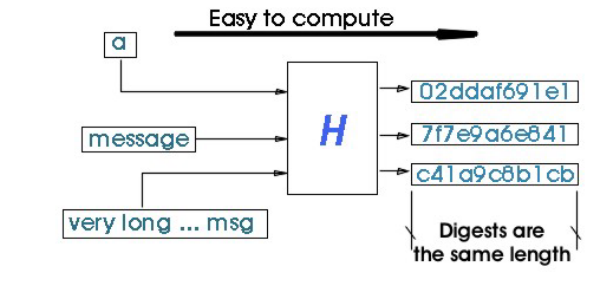
\includegraphics[width=1\textwidth]{images/hash_function.png}
  \caption[Hash function]{Hash function}
  \label{fig:hash_function}
\end{figure}

According to NIST, a cryptographic hash mush satisfied following three properties:

\begin{itemize}
  \item Collision resistance: It is computationally infeasible to find two inputs that have the same hash value. The most efficient method to find must be brute-forcing of random inputs. The birthday ”paradox” places an upper bound on collision resistance. That is, the complexity (or collision-resistance strength) of seeking two different inputs $M$ and $M^{\prime}$ matched two hash $H(x) = H(x^{\prime})$ equal to $L/2$ bit-operations for a $L$-bit hash function. For example, SHA-512 produces a collision resistance of 256 bits.

  \item Preimage resistance: Given a hash value h, it is computationally infeasible to find an $M$ that $H(M)=h$. Preimage resistance strength is equal to the amount of work to brute-force $L$-bit of operations for an $L$-bit hash function. For example, SHA-512 provides a preimage resistance of 512 bits.

  \item Second preimage resistance: Finding a second input that has the same hash value as any other specified input would be computationally infeasible. Second preimage resistance is calculated by the number of operations equal to $L$ bits for an $L$-bit hash function. For example, SHA-512 produces a (full-length) hash value of 512 bits. However, in some cases of the hash functions, the second preimage resistance also depends on the length of the message resulting from the hash function.
\end{itemize}


\subsubsection{Secure Hash Algorithm with digest 512 bits (SHA-512)}

The SHA-512 may be used to hash a message $M$ having a length of l bits, where $l \leq 0 \leq 2^{128}$. It produces a result of 512-bit message digest. The SHA-512 is part of a group of hashing algorithms that are very similar in how they work, called SHA-2. Algorithms such as SHA-256 are a part of this group alongside SHA-512. SHA-256 is used in blockchain as the default hash function. In our thesis, SHA-512 and SHA-256 will be used in the key derivation algorithm.

\subsubsection{Hash-based message authentication codes (HMACs)}

HMACs are a tool for calculating message authentication codes using a cryptographic hash function coupled with a secret key. HMAC can provide message authentication using a shared secret instead of using digital signatures with asymmetric cryptography. NIST mentioned in \href{https://nvlpubs.nist.gov/nistpubs/FIPS/NIST.FIPS.198-1.pdf}{FIPS.198-1} that HMAC uses a key, $K$, of appropriate security strength, compute with a text using the operation as follows:
\vspace{0.2cm}
\begin{center}
  $HMAC(K, text) = H((K_0 \oplus opad )\| H((K_0 \oplus ipad) \| text))$
\end{center}
\vspace{0.2cm}

Where:

\begin{itemize}
  \item $H$ is a cryptographic hash function (our thesis use SHA-512 and SHA-256)
  \item $text$ is the data
  \item $K$ is the secret key
  \item $K_0$ is a key derived from the secret key by padding to the right with 0s up to the block size, or by hashing down to less than or equal to the block size first and then padding to the right with zeros
  \item $\oplus$ denotes bitwise exclusive or (XOR)
  \item $opad$ is a block size repeated bytes $0x5c$
  \item $ipad$ is a block size repeated bytes $0x36$
\end{itemize}

The final result of HMAC is equivalent to that of the underlying hash function (for example, 256 and 512 bits respectively in the case of SHA-256 and SHA-512), although it can be truncated if desired.

\subsection{Password Based Key Derivation Function (PBKDF2)}

PBKDF2 is a simple cryptographic key derivation function approved by NIST, which is resistant to dictionary attacks and rainbow table attacks (use precomputed hashes). It applies a pseudorandom function (our thesis uses HMAC) to the input password or passphrase along with a salt value and repeats the process many times to produce a derived key, which can then be used as a cryptographic key in subsequent operations. PBKDF2 takes several input parameters and produces the derived key as output:

\vspace{0.2cm}
\begin{center}
  $key = pbkdf2(password, salt, iteration, h, k)$
\end{center}
\vspace{0.2cm}

Technically, the input data for PBKDF2 consists of:

\begin{itemize}
  \item A $password$ - array of bytes / string, e.g. “stronger mnemonic”
  \item A $salt$ - array of bytes / string generated by approved Random Bit Generator, e.g. "stronger password" (minimum 64 bits, NIST recommended 128 bits is optimal)
  \item The $iteration$, e.g. 100000 iterations
  \item $h$: a hash function for calculating HMAC, e.g. SHA256
  \item $k$: key-length size, e.g. 32 bytes (256 bits)
\end{itemize}



